% Chapter 3

\chapter{Construction} % Write in your own Chapter title
\label{Chapter3}
%contain a description of the program that the students have created, what choices they have made during development and why they have made those choices.

\section{Introduction}

\cite  {SoftwE}

\section{Tools}
This section is about the different tools used during the construction of the app.

\subsection{Version Control}\label{verCon}
Git was used as the version control during the development of the app. It was chosen because the developer already knew how to use it. GitHub for windows was used to backup the project. The full GitHub project is available online \cite{detemegandy}.
 
\subsection{The Android Operating System }
Android {OS} is the mobile operating system with the largest market share at the time of this writing\cite{gartner}. Android will be celebrating its 10 year anniversary on September 23, 2018\cite{android_developers_blog_2008}. Figure \ref{android-stack} shows the major components of the Android platform. The two official programming languages of Android applications are Kotlin and Java, the latter being most used today. The OS is open source, and anyone can contribute to the development\cite{android_open_source_project}.

\begin{figure}[!htb]
 \centering
 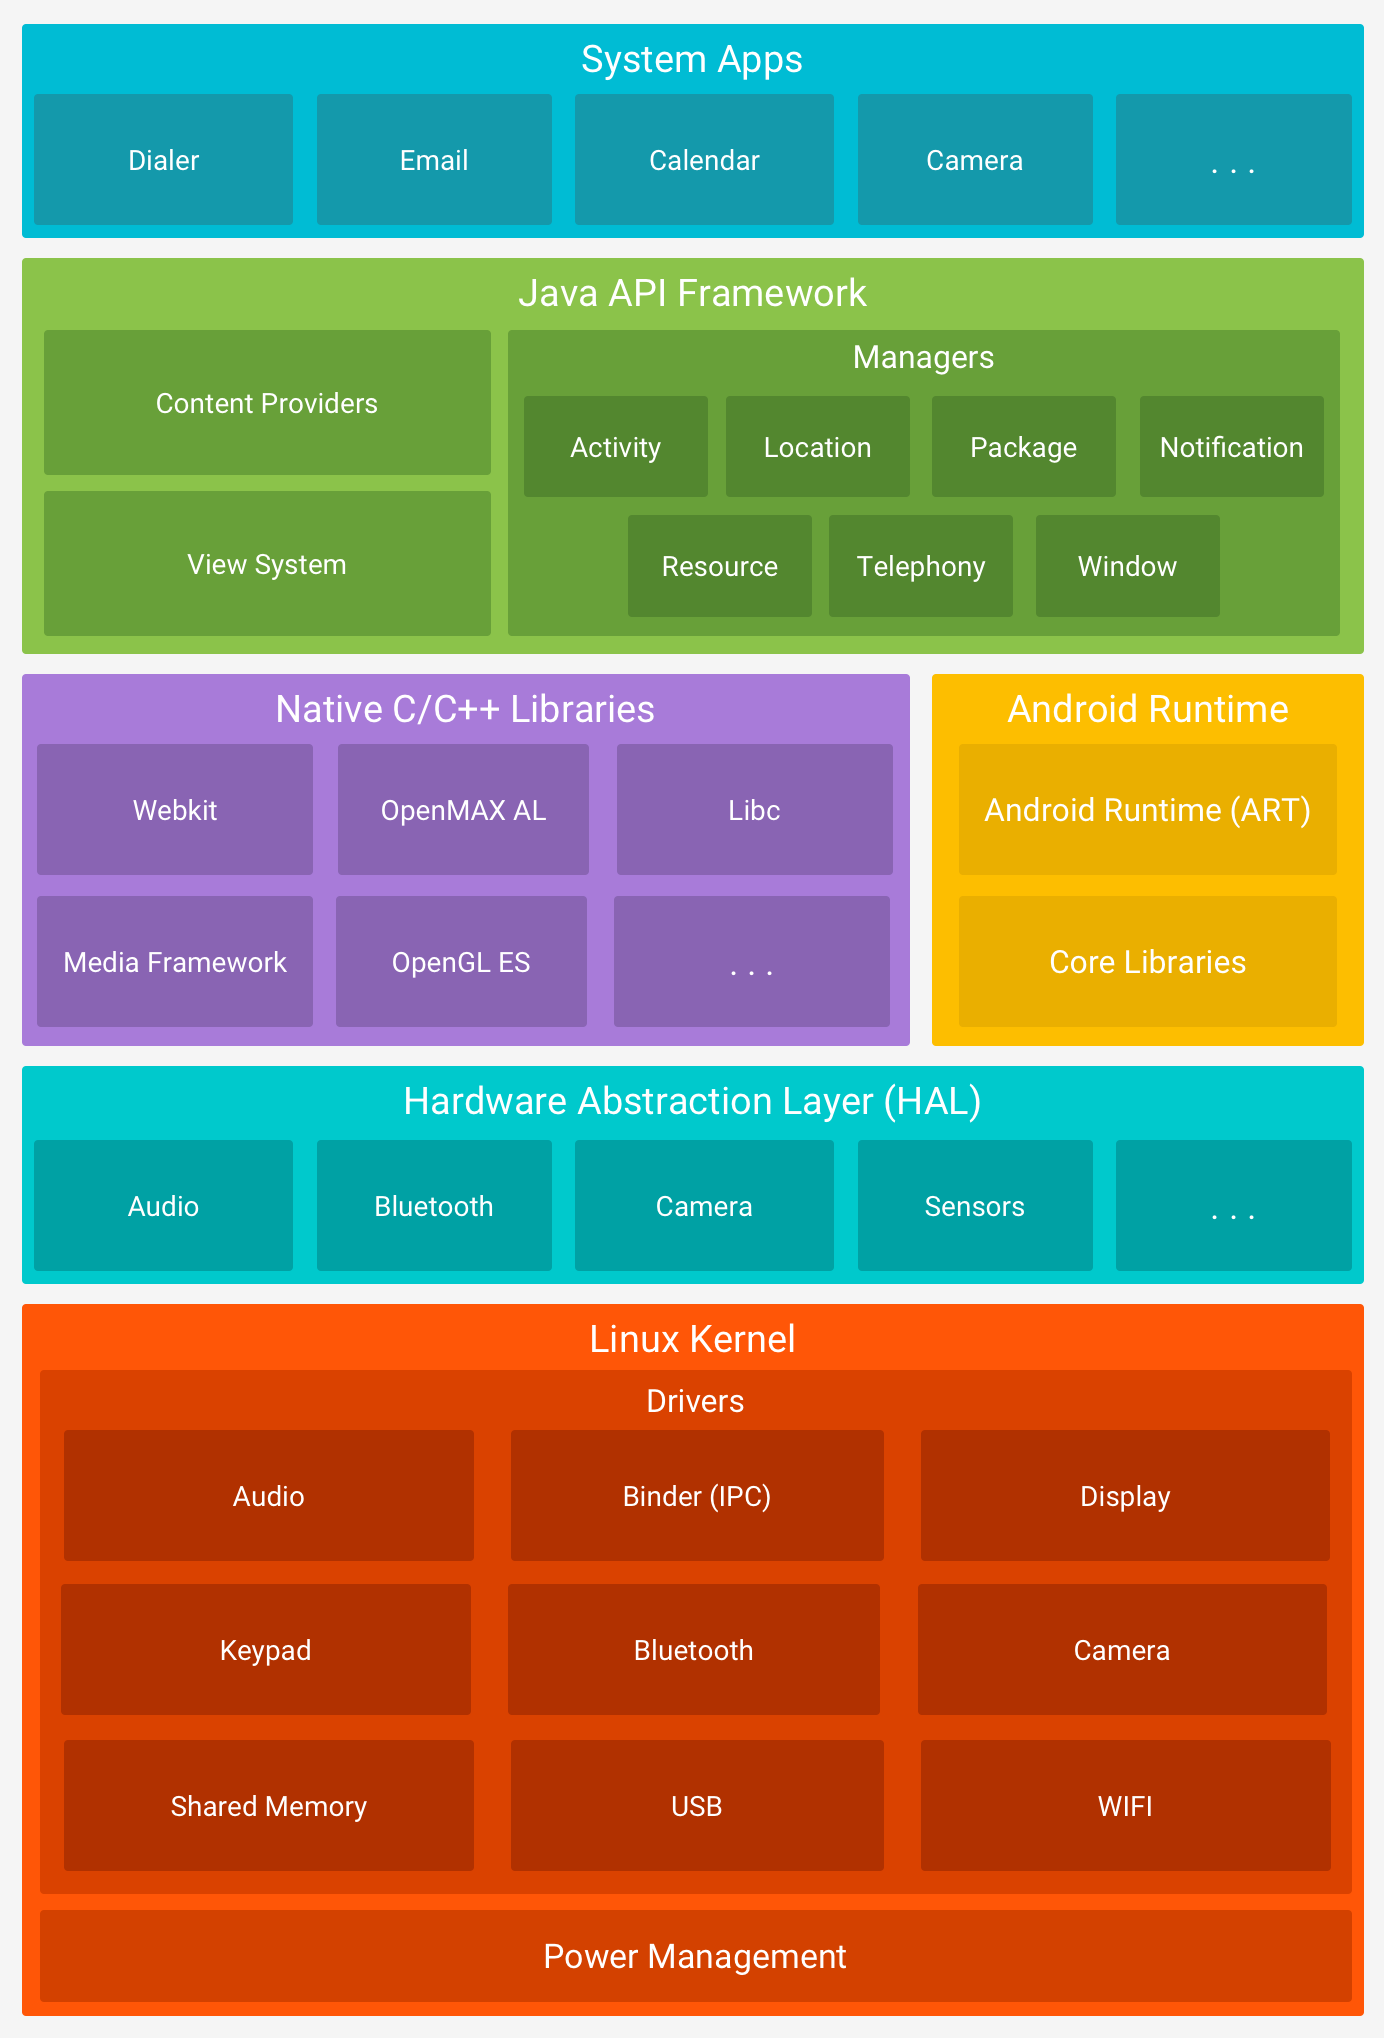
\includegraphics[width=\linewidth]{android-stack_2x.png}
 \caption{The Android software stack \label{android-stack} \cite{android_developers_2018}}
\end{figure}

\subsubsection{The Linux Kernel}
"The foundation of the Android platform is the Linux kernel. For example, the Android Runtime (ART) relies on the Linux kernel for underlying functionalities such as threading and low-level memory management.
Using a Linux kernel allows Android to take advantage of key security features and device manufacturers to develop hardware drivers for a well-known kernel."~\cite{android_developers_2018}


\subsubsection{Android Runtime}
"For devices running Android version 5.0 (API level 21) or higher, each app runs in its own process and with its own instance of the Android Runtime (ART). Some of the major features of ART include the following:

\begin{itemize}
 \item Ahead-of-time (AOT) and just-in-time (JIT) compilation
 \item Optimized garbage collection (GC)
 \item Better debugging support, including a dedicated sampling profiler, detailed diagnostic exceptions and crash reporting, and the ability to set watchpoints to monitor specific fields...
\end{itemize}
  
Android also includes a set of core runtime libraries that provide most of the functionality of the Java programming language, including some Java 8 language features, that the Java API framework uses."~\cite{android_developers_2018}
 
 \subsubsection{Java API Framework}
 "The entire feature-set of the Android OS is available through APIs written in the Java language. These APIs form the building blocks you need to create Android apps by simplifying the reuse of core, modular system components and services, which include the following:
 
 \begin{itemize}	
 	\item A rich and extensible View System you can use to build an app’s UI, including lists, grids, text boxes, buttons, and even an embeddable web browser
 	\item A Resource Manager, providing access to non-code resources such as localized strings, graphics, and layout files
 	\item A Notification Manager that enables all apps to display custom alerts in the status bar
 	\item An Activity Manager that manages the lifecycle of apps and provides a common navigation back stack
 	\item Content Providers that enable apps to access data from other apps, such as the Contacts app, or to share their own data	
 \end{itemize}

 Developers have full access to the same framework APIs that Android system apps use."~\cite{android_developers_2018}
 
 
 \subsection{Android Studio}
 
 \begin{figure}[!htb]
 	\centering
 	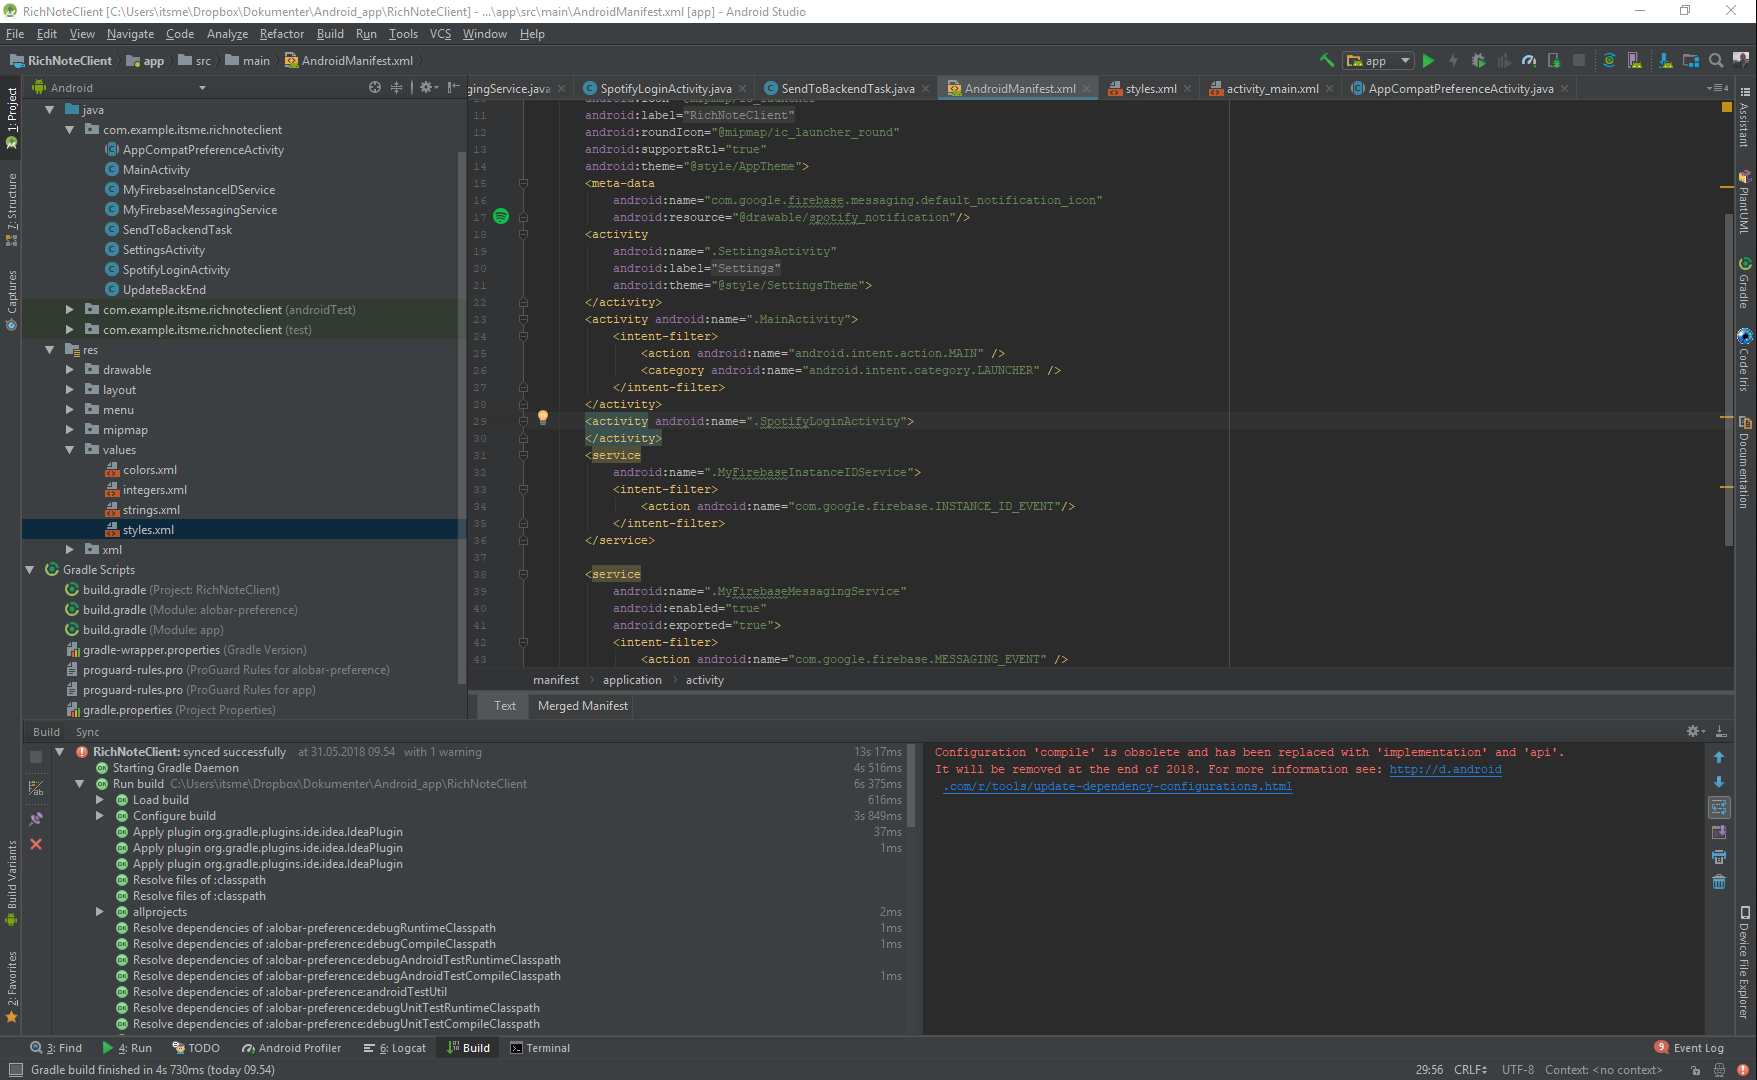
\includegraphics[width=\linewidth]{android-studio.png}
 	\caption{Android Studio \label{android-studio}}
 \end{figure}
"Android Studio is the official Integrated Development Environment (IDE) for Android app development, based on IntelliJ IDEA . On top of IntelliJ's powerful code editor and developer tools, Android Studio offers even more features that enhance your productivity when building Android apps, such as:
\begin{itemize}
\item A flexible Gradle-based build system
\item A fast and feature-rich emulator
\item A unified environment where you can develop for all Android devices
\item Instant Run to push changes to your running app without building a new APK
\item Code templates and GitHub integration to help you build common app features and import sample code
\item Extensive testing tools and frameworks
\item Lint tools to catch performance, usability, version compatibility, and other problems
\item C++ and NDK support
\item Built-in support for Google Cloud Platform, making it easy to integrate Google Cloud Messaging and App Engine"\cite{android_studio}
\end{itemize}
 \subsection{Gradle}
 The flexible Gradle-based build system is so well integrated, that you barely have to know anything about it to use Android Studio. However when it fails to parse some of the dependencies of the project, it can get time consuming. During the development of the application the upgrade of android studio would sometimes break the project. A complete removal and reimporting av the project would be needed to continue development. Three files relating to Gradle where edited without automation. The project build.gradle file, the app build.gradle file and the settings.gradle file. They were edited to set minimum android SDK versions, add directory with the alobar-preference\cite{alobar} library that was used in the SettingsActivity.\ref{settingsactivity}
 
 \subsection{Firebase Cloud Messaging}
 Firebase Cloud Messaging (FCM) was chosen as the delivery service for the notifications coming from the backend. This was chosen because it is free and also developed by Google\cite{FCM}.
\section{Code}

\subsection{The App Manifest ~\cite{appManifest}}
Every app project must have an AndroidManifest.xml file (with precisely that name) at the root of the project source set. The manifest file describes essential information about your app to the Android build tools, the Android operating system, and Google Play.

Among many other things, the manifest file is required to declare the following:
\begin{itemize}
	\item The app's package name, which usually matches your code's namespace. The Android build tools use this to determine the location of code entities when building your project. When packaging the app, the build tools replace this value with the application ID from the Gradle build files, which is used as the unique app identifier on the system and on Google Play. 
\item The components of the app, which include all activities, services, broadcast receivers, and content providers. Each component must define basic properties such as the name of its Kotlin or Java class. It can also declare capabilities such as which device configurations it can handle, and intent filters that describe how the component can be started.

\item The permissions that the app needs in order to access protected parts of the system or other apps. It also declares any permissions that other apps must have if they want to access content from this app. 

\item The hardware and software features the app requires, which affects which devices can install the app from Google Play. \end{itemize}

The app manifest is shown in listing \ref{appManifest}
\clearpage
\begin{lstlisting}[language=XML, caption={app manifest},label={appManifest}]
<manifest xmlns:android="http://schemas.android.com/apk/res/android"
package="com.example.itsme.richnoteclient">
<uses-permission android:name="android.permission.ACCESS_NETWORK_STATE" />
<uses-permission android:name="android.permission.INTERNET" />
<uses-permission android:name="android.permission.READ_PHONE_STATE"/>
<application
    android:allowBackup="true"
    android:icon="@mipmap/ic_launcher"
    android:label="@string/app_name"
    android:roundIcon="@mipmap/ic_launcher_round"
    android:supportsRtl="true"
    android:theme="@style/AppTheme">
    <meta-data
    android:name="com.google.firebase.messaging.default_notification_icon"
    android:resource="@drawable/spotify_notification"/>
    <activity
        android:name=".SettingsActivity"
        android:label="@string/SettingsActivityName"
        android:theme="@style/SettingsTheme">
    </activity>
    <activity android:name=".MainActivity">
        <intent-filter>
            <action android:name="android.intent.action.MAIN" />
            <category android:name="android.intent.category.LAUNCHER" />
        </intent-filter>
    </activity>
    <activity android:name=".SpotifyLoginActivity">
    </activity>
    <service
        android:name=".MyFirebaseInstanceIDService">
        <intent-filter>
            <action android:name="com.google.firebase.INSTANCE_ID_EVENT"/>
        </intent-filter>
    </service>
    <service
        android:name=".MyFirebaseMessagingService"
        android:enabled="true"
        android:exported="true">
    <intent-filter>
        <action android:name="com.google.firebase.MESSAGING_EVENT" />
        <action android:name="com.firebase.jobdispatcher.ACTION_EXECUTE" />
    </intent-filter>
    </service>
</application>
</manifest>
\end{lstlisting}

The first two lines in the app manifest are automatically generated my Android Studio. These lines are used by the Android Runtime Environment(ARE), the first line to uniquely identify elements in the rest of the manifest, the second to uniquely identify classes in the project. The next few lines declares permissions that the app uses in some of its classes.

\subsubsection{Permissions \cite{permissions}}{
Permissions are part of the android Application Programming Interface (API). The purpose of a permission is to protect the privacy of an Android user. Android apps must request permission to access sensitive user data (such as contacts and SMS), as well as certain system features (such as camera and internet). Depending on the feature, the system might grant the permission automatically or might prompt the user to approve the request. Some permissions are never granted to 3rd party apps.}

\begin{figure}[!htb]
	\centering
	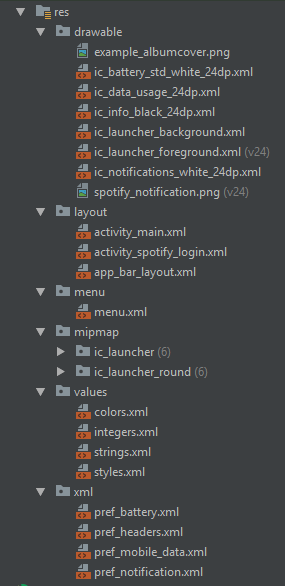
\includegraphics[height=\textheight/2]{resources.png}
	\caption{The App Res folder \label{resourceFolder} }
\end{figure} 

The first two permissions are self-explanatory. The app needs internet to communicate with the backend, and access of the devices network state to monitor the type of connectivity currently in use. The permission in line 6 is a in a group that is labeled by Google as dangerous. This means that the app has to ask the user for this permission using a dialog at runtime. More about this in the MainActivity class \ref{mainactivity}. This permission is used to acquire a identification(ID) that comes from the physical sim-card in the phone. This ID is used in the UpdateBackend class \ref{updatebackend}. From line 7 onward, the lines are inside the application tag. This means we only affect the application with the next lines. The preceding lines affected the package, which could have several applications in it. Since the app is not published on the Google Play store, line 8 has no effect on the application. In lines 9 through 13, resources from the Res directory of the project is referenced. In the resources directory there are things that are used depending on the characteristics of the device the application is deployed on. IE there would be different sizes of the images used for the launcher icons that are displayed on the home screen of the device, depending on the size of the screen. The app's resource folder is pictured in figure \ref{resourceFolder}. Further in the manifest we assign the launcher and round icon of the app. One of these are used depending on the version of android running on the device. The services and meta data tags later are added by requirements to use the FCM service.

\subsubsection{AppTheme}
\begin{lstlisting}[language=XML, caption={styles.xml},label={styles}]
<resources>
<!-- Base application theme. -->
<style name="AppTheme" parent="Theme.AppCompat.NoActionBar">
<!-- Customize your theme here. -->
<item name="colorPrimary">@color/colorPrimary</item>
<item name="colorPrimaryDark">@color/colorPrimaryDark</item>
<item name="colorAccent">@color/colorAccent</item>
</style>
<style name="SettingsTheme" parent="Theme.AppCompat">
<item name="colorPrimary">@color/colorPrimary</item>
<item name="colorPrimaryDark">@color/colorPrimaryDark</item>
<item name="colorAccent">@color/colorAccent</item>
</style>
</resources>
\end{lstlisting}
We assign the colors and the app class in line 12. We get it from the styles XML file. The theme is set to AppCompat's subclass NoActionBar which is a application class that has backwards compatibility and no actionbar. This is done to enable the addition of the appCompatActionbar in the MainActivity class which also has backwards compatibility. The settings theme in the styles.xml file is used for the SettingsActivity. You can view the styles.xml in listing \ref{styles}. The remaining lines in the Manifest declare the MainActivity Intent-filters and the SpotifyLoginActivity. 

\subsection{MainActivity \label{mainactivity}}
the MainActivity is the first class where code gets executed on android applications. It is analogues to the main method in Java. The reason for this is the registered intent-filter from the manifest.
\begin{figure}[!htb]
	\centering
	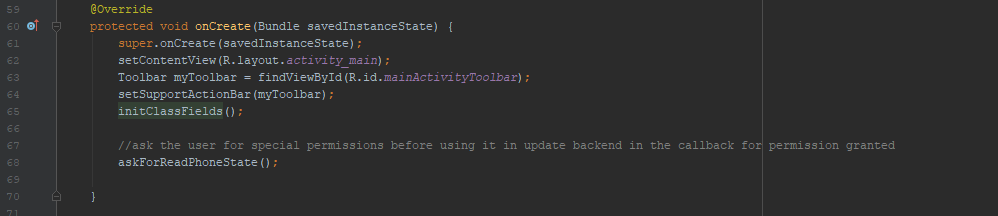
\includegraphics[width=\linewidth]{mainoncreate.png}
	\caption{MainActivity's onCreate method \label{mainoncreate} }
\end{figure}

\subsubsection{Intents and Intent-filters}
Intents are basically a way to send data too, and receive data from, other activities or services. The filters are used to filter which intents actually gets through to the activity\cite{intent}.

\subsubsection{Activity}
"The Activity class is a crucial component of an Android app, and the way activities are launched and put together is a fundamental part of the platform's application model. Unlike programming paradigms in which apps are launched with a main() method, the Android system initiates code in an Activity instance by invoking specific callback methods that correspond to specific stages of its lifecycle. Over the course of its lifetime, an activity goes through a number of states. You use a series of callbacks to handle transitions between states."\cite{activity} 


\begin{figure}
	\centering
	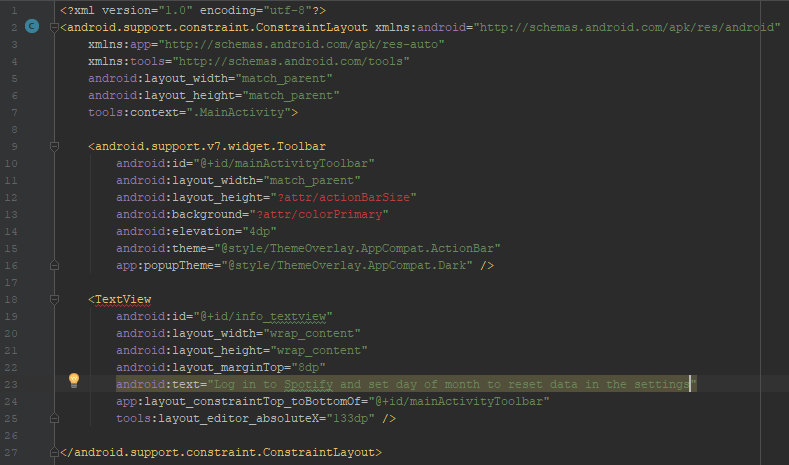
\includegraphics[width=1\linewidth]{Figures/activity_main}
	\caption{Main Activity Layout file}
	\label{fig:activitymain}
\end{figure}


You must implement the onCreate callback in every activity. In MainActivity's creation we set the layout to the activity\_main XML file. In this layout we have added the toolbar to show the app name and menu items. There is also a Text View used to give a new user a brief setup manual. You can read the manual in figure \ref{fig:activitymain}. Then the toolbar is added and this triggers the onCreateOptionsMenu callback. In the override of this method we use a API call to inflate the menu declared in the menu XML file. We also make sure to remove the Spotify log in option if the user has previously logged inn. After menu has been added, the initClassFields method is called. In the initialization method the get the text view by its id, which we access from the strings XML file. We also make use of the Android API to get access to a file where we can store and retrieve key-value pairs on persistent storage. Using the file we check if the user has logged in to Spotify.

The items in the menu have an event listener that gets triggered should the user click them. This method is called on option item selected. In the method we launch the Spotify log in activity and register the main activity for a to a callback function when the spotify activity has finished.

The callback uses the intent parameter and checks if the user is logged in. If the user is logged in, the menu gets created again so that the menu item for logging in is set to invisible. See the complete code in figure \ref{fig:mainonactivityresult}.
\begin{figure}
	\centering
	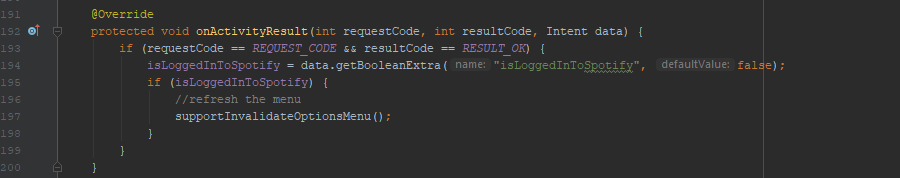
\includegraphics[width=1\linewidth]{Figures/mainonactivityresult}
	\caption{on activity result callback method in main activity}
	\label{fig:mainonactivityresult}
\end{figure}

The final lines in main activity prompts the user for the permission to read the phone state. This permission is needed to retrieve mobile data usage of the application. When the dialog is closed, a check for permission granted is performed. If we have the permission we schedule to update the backend periodically. This is done with the newly released WorkManager API. It guaranties code execution that was planned, energy efficiently, in the background on another thread. The User Interface is not stalled by this, since it runs on a different thread. The update is scheduled to run once every 30-60 minutes. It only runs if the device has a Internet connection available. It passes the UdateBackend worker class to a work request, which is enqueued with the Workmanager system service.



\subsection{UpdateBackend \label{updatebackend}}
UpdateBackend is an extension of the Worker class from the Workmanager API. The algoriths in it refreshes the constraints on the backend. It puts the data in a json string and sends it to the backend via http POST request. 
\subsection{SettingsActivity \label{settingsactivity}}
The settings activity is mostly generated by the IDE using a creation dialog. A number picker preference is added from the alobar library imported with gradle. It has eventlisteners for preference changes, and stores values in the same file retrieved in the main activity class in the initialize method.
\subsection{FCM}
Firebase messaging is implemented with the extension of the FirebaseInstanceIdService, to listen for unique identifiers of the installation of the app. This is sent to the backend and a response with a unique spotify url is given in response from the server. This is used in a webview to open a dialog with Spotify so the user can log in. This is leaves the security concerns to the Spotify oauth API implemetation.

The extension of the Firebasemessagingservice is used to receive messages that can wake up the device and execute code in the background in spite of new restrictions imposed by the latest android version: OREO. Here notifications are prepared and then sent to the system notification service provided by android. Standard layouts are used.